\chapter{Sistemas de ficheros a analizar}\label{sec:capítulo_3}

\section{¿Por qué hemos elegido estos sistemas de ficheros?}

Medir el uso de los sistemas de ficheros es una tarea desafiante debido a la falta de estudios exhaustivos que recojan esta información de manera global. Ante esta dificultad, hemos optado por obtener el listado de las 64 distribuciones más descargadas en 2023 y analizar los sistemas de ficheros que soportan por defecto. La figura \ref{fig:uso sistemas de ficheros}, derivada de la tabla referenciada en el \nameref{sec:anexo}, nos proporciona una visión clara de la distribución del uso de sistemas de ficheros en estas distribuciones.

\begin{figure}[htbp]
    \centering
    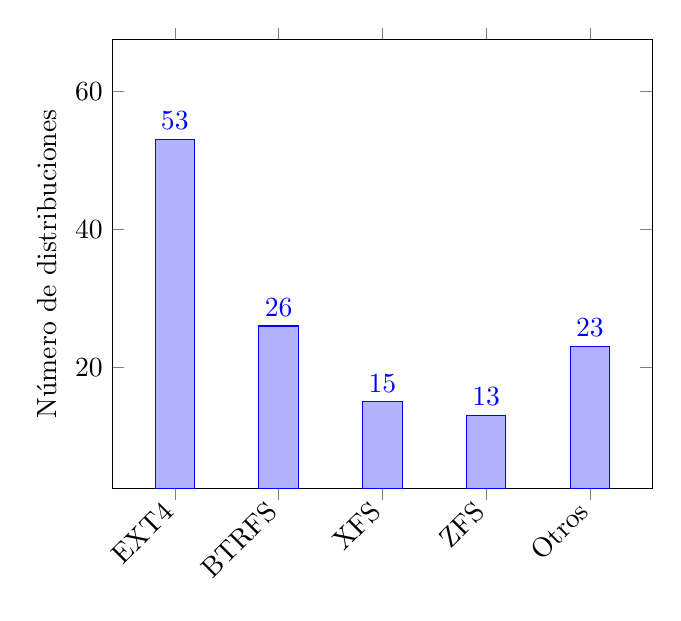
\begin{tikzpicture}
        \begin{axis}[
            ybar,
            bar width=0.5cm,
            enlargelimits=0.15,
            ylabel={Número de distribuciones},
            xticklabels={EXT4, BTRFS, XFS, ZFS, Otros},
            xtick=data,
            nodes near coords,
            nodes near coords align={vertical},
            ymode=normal,
            ymin=10,
            ymax=60,
            x tick label style={rotate=45,anchor=east},
            ]
            \addplot coordinates {(0, 53) (1, 26) (2, 15) (3, 13) (4, 23)};
        \end{axis}
    \end{tikzpicture}
    \caption{Sistemas de ficheros más usados en 2023}
    \label{fig:uso sistemas de ficheros}
\end{figure}

Hemos seleccionado los sistemas de ficheros que estas distribuciones utilizan como predeterminados, entre los cuales se encuentran EXT4, BTRFS, XFS y ZFS. Estos sistemas no solo destacan por su amplio uso, sino también por su madurez y relevancia en el panorama actual de los sistemas de ficheros para Linux. Cada uno de ellos ofrece un conjunto único de características y funcionalidades que los hacen atractivos y confiables para diferentes aplicaciones y entornos de trabajo.

Entender la cronología de estos sistemas de ficheros es esencial para obtener una comprensión completa de su evolución y comprender cómo han llegado a ser lo que son en la actualidad. Con esta selección, no solo buscamos comprender las tendencias actuales en el uso de sistemas de ficheros en entornos Linux, sino también analizar detenidamente las características y capacidades de los sistemas más relevantes.

\begin{figure}[h!]
    \centering
    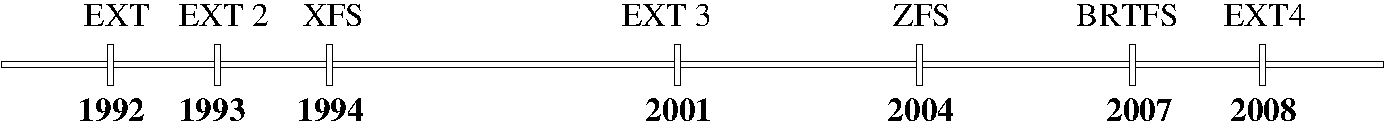
\includegraphics[width=1\linewidth]{figures/timeline.pdf}
    \caption{Línea de tiempo de los sistemas de ficheros de Linux}
    \label{fig:linea tiempo fs}
\end{figure}

El linaje de EXT4 se remonta a los primeros días del sistema de ficheros EXT, que apareció en 1992. Posteriormente, en 1993, se introdujo EXT2 como una mejora significativa, seguido por EXT3 en 2001, que ofrecía mejoras adicionales. Sin embargo, fue con la llegada de EXT4 en 2008, introducido en el kernel Linux 2.6.28, que el sistema de ficheros EXT alcanzó su punto más alto en términos de rendimiento, confiabilidad y capacidades avanzadas.

XFS, por otro lado, tiene sus raíces en los esfuerzos de Silicon Graphics Inc. (SGI) en 1994. Desarrollado como un sistema de ficheros de alto rendimiento para el sistema operativo IRIX, XFS se adaptó a Linux y se convirtió en una opción popular para aplicaciones que requieren un manejo eficiente de grandes volúmenes de datos. XFS se incorporó al kernel Linux en la versión 2.1.47, lanzada en 1997.

El surgimiento de BTRFS en 2007 marcó un hito en el desarrollo de sistemas de ficheros para Linux. Anunciado como un proyecto experimental, BTRFS fue concebido como un sistema de ficheros de próxima generación, que terminó siendo introducido en el kernel de Linux en la versión 2.6.29, lanzada en 2009.

ZFS, diseñado por Sun Microsystems en 2004, inicialmente para el sistema operativo Solaris, ha sido adoptado en entornos Linux mediante implementaciones de código abierto. Sin embargo, debido a diferencias de licencia entre la Licencia Pública General de GNU (GPL) utilizada por el kernel de Linux y la Licencia de Sun CDDL utilizada por ZFS, la integración oficial de ZFS en el kernel de Linux no se ha producido. En su lugar, existen proyectos de código abierto como OpenZFS que permiten utilizar ZFS en sistemas Linux.

\section{EXT4 (Extended File System 4)}

El sistema de ficheros EXT4 es uno de los sistemas de ficheros más utilizados en el entorno Linux debido a su robustez, eficiencia y capacidad para manejar grandes volúmenes de datos. Para comprender completamente cómo funciona EXT4, es crucial explorar su estructura interna y sus principales características.

\subsection{Estructura interna de EXT4}

\begin{figure}[h!]
    \centering
    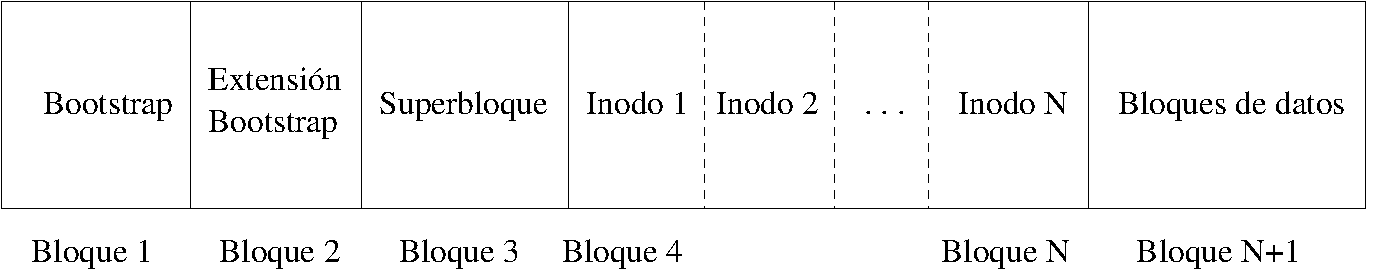
\includegraphics[width=0.85\linewidth]{figures/ext4.pdf}
    \caption{Estructura interna de EXT4}
    \label{fig:estructura interna de EXT4}
\end{figure}

La figura \ref{fig:estructura interna de EXT4} muestra la estructura interna del sistema de ficheros EXT4, que comparte la base de sus predecesores como EXT, EXT2 y EXT3 \cite{ext4-wiki,ext4_current_status,anatomy_ext4}. Esta estructura se compone de los siguientes elementos:

\begin{enumerate}
    \item \textbf{Arranque (Bootstrap):} El arranque se refiere al proceso inicial de carga del sistema operativo durante el inicio del sistema. En este proceso, se lleva a cabo la rutina de carga del kernel en memoria y una inicialización básica del hardware. Si no hay un cargador de arranque sofisticado como el GRUB, el kernel debe encontrarse en una posición fija en disco; de lo contrario, el cargador determina la partición y forma de arranque. Además, debe reconocer el formato del sistema de ficheros de arranque.

    \item \textbf{Extensión del Bootstrap:} Esta sección contiene datos adicionales necesarios para el arranque del sistema operativo, como la rutina llamada "setup" que termina la configuración del hardware. En EXT4, se incluyen mejoras en la eficiencia y rapidez de este proceso gracias a optimizaciones en la gestión de los metadatos y la estructura de almacenamiento.

    \item \textbf{Superbloque:} El superbloque es una estructura de metadatos que contiene información crucial sobre el sistema de ficheros EXT4. En este sistema de ficheros, el superbloque incluye elementos adicionales como referencias a los extents y timestamps necesarios para la optimización del acceso a los datos.
    
    \item \textbf{Lista de inodos:} Como ya hemos comentado previamente, los inodos son estructuras de datos que almacenan información sobre archivos, directorios y pipes en el sistema de ficheros. En EXT4, la lista de inodos secuencial permite un acceso más eficiente que sus antecesores.
    
    \item \textbf{Bloques de datos:} Los bloques de datos constituyen la parte principal del sistema de ficheros EXT4, ya que almacenan el contenido real de archivos, pipes y directorios. Estos bloques contienen una variedad de datos, incluyendo texto, imágenes gráficas en diferentes formatos, archivos binarios, entre otros.
\end{enumerate}

\subsection{Características de EXT4}

En cuanto a las características mencionadas anteriormente en la sección \ref{sec:caracteristicas_principales_sistemas_ficheros}, el sistema de ficheros EXT4 incluye características fundamentales como journaling, registrando las transacciones sobre el sistema de ficheros para garantizar la integridad de los datos en caso de fallos del sistema. Sin embargo, no ofrece soporte nativo para snapshots, \textit{copy on write}, compresión o deduplicación. En cambio, EXT4 cuenta con características que lo hacen único cómo son:

\textbf{Compatibilidad y retrocompatibilidad:} Fue diseñado específicamente para ser lo más compatible posible con EXT3, permitiendo la actualización in situ de sistemas de ficheros existentes previos como EXT3 y EXT2, así como el montaje automático de los mismos.\newline

\textbf{Grandes sistemas de ficheros:} EXT4 superó las limitaciones de direccionamiento de 32 bits de EXT3 mediante el uso de direccionamiento interno de 48 bits, permitiendo ficheros cuyo tamaño máximo es de 16 TiB, sobre un sistema de ficheros que en conjunto puede tener hasta 1 EiB.\newline

\textbf{Extents:} La implementación de extents simplifica la asignación y gestión de bloques físicos consecutivos, lo que resulta en una reducción del tamaño de la tabla de asignación. Aunque el espacio ocupado por el inodo permanece invariable, la adopción de bloques consecutivos simplifica las estructuras de almacenamiento necesarias para archivos grandes, reduciendo así el espacio requerido por estas tablas. Además de mitigar la fragmentación, esta mejora en la organización del almacenamiento también optimiza las operaciones de lectura.\newline

\textbf{Preasignación persistente:} Esta característica busca eliminar la necesidad de "blanquear" un bloque de datos con ceros cada vez que se asigna a un fichero, una operación comúnmente realizada para borrar su contenido anterior. En su lugar, el sistema hace uso de un "pool" de bloques previamente blanqueados, lo que agiliza la expansión de ficheros. En la práctica, esta mejora de rendimiento se evidencia en todas las situaciones, especialmente durante escrituras intensivas sobre el fichero.

\section{BTRFS (B-tree File System)}

BTRFS (B-tree File System) es un sistema de ficheros moderno, diseñado para ofrecer características avanzadas de gestión de almacenamiento de datos en entornos Linux. A diferencia de algunos sistemas de ficheros tradicionales, como EXT4, BTRFS utiliza una estructura de árbol B (B-tree) para organizar y gestionar los datos en el disco \cite{btrfs-docs,btrfs_design,btrfs_get_started,btrfs_swiss_army_knife}.

\begin{figure}[h!]
    \centering
    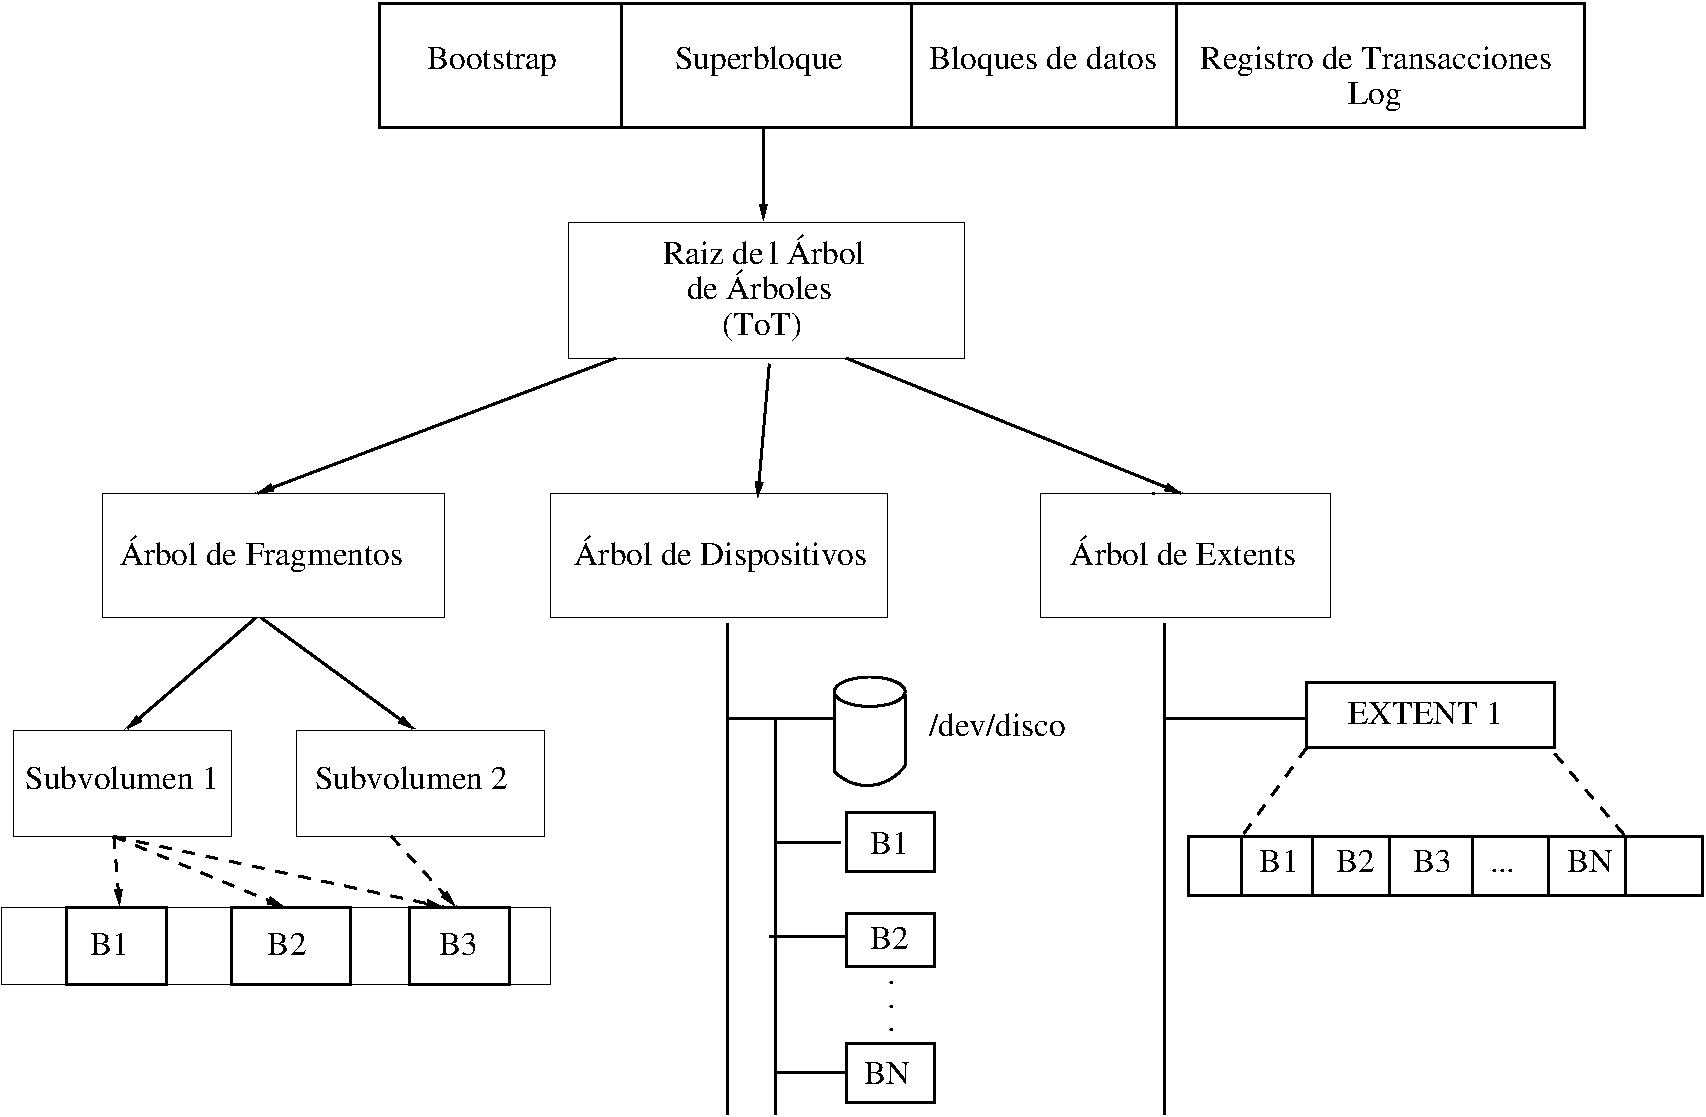
\includegraphics[width=1\linewidth]{figures/btrfs_btree.pdf}
    \caption{Estructura del superbloque en BTRFS}
    \label{fig:BTRFS-superblock}
\end{figure}

\subsection{Estructura interna de BTRFS}

Como podemos ver en la figura \ref{fig:BTRFS-superblock}, BTRFS presenta una estructura de sistema de ficheros más compleja en comparación con los sistemas EXT y sus extensiones, debido al uso que hace de árboles-B y funciones de hashing para almacenar la información.

En este contexto, el superbloque desempeña un papel fundamental al referenciar estructuras cruciales del disco. El superbloque contiene varias estructuras de datos que permiten organizar el almacenamiento de una forma muy eficiente, sobre todo de cara a acceder a la información. Estas estructuras de datos tienen una representación de árbol y son las siguientes:

\begin{itemize}
    \item \textbf{Raíz del árbol de árboles (TOT):} Es la raíz del árbol de metadatos en BTRFS. Contiene referencias a otros árboles importantes, como el árbol de fragmentos, el árbol de gestión de dispositivos y el árbol de almacenamiento por grupos de bloques. Es esencial para la navegación y la gestión del sistema de ficheros.
    
    \item \textbf{Árbol de fragmentos:} Este árbol organiza y gestiona los fragmentos de datos en el disco. Los fragmentos son bloques de datos físicos de tamaño fijo que se asignan dinámicamente para almacenar archivos y metadatos.
    
    \item \textbf{Árbol de gestión de dispositivos:} Este árbol nos permite conocer en qué dispositivos de almacenamiento tenemos representados los diferentes bloques de datos. Persigue una distribución eficiente del almacenamiento entre los dispositivos disponibles, gestionando cómo se asignan los bloques de datos a cada dispositivo.
    
    \item \textbf{Árbol de almacenamiento por grupos de bloques (extents):} Organiza los bloques de datos en grupos contiguos llamados "extents". Cada extent representa una región de bloques de datos consecutivos en el disco y se utiliza para asignar espacio a archivos y directorios en el sistema de ficheros BTRFS.
\end{itemize}

En BTRFS, es importante destacar que los inodos no se enumeran directamente después del superbloque, como suele ser el caso en otros sistemas de ficheros. En su lugar, se almacenan dentro del árbol de fragmentos. Esta implementación tiene la ventaja de agilizar la localización de los inodos mediante el uso de una estructura arborescente.

\subsection{Características de BTRFS}

BTRFS presenta características clave como \textit{copy on write}, snapshots y compresión y descompresión integradas, explicadas en la sección \ref{sec:caracteristicas_principales_sistemas_ficheros}. A continuación, resaltaremos algunas de las características específicas de BTRFS:

\textbf{Escritura retrasada:} La estrategia consiste en emplear la escritura diferida para agrupar un conjunto de escrituras consecutivas sobre un fichero en bloques posiblemente consecutivos, con el objetivo de reducir la fragmentación y mejorar el rendimiento. Esto se logra mediante el uso de los cachés de disco, que permiten acceder y utilizar esta información de forma rápida en la memoria principal antes de que se escriba en disco unos segundos más tarde. Para archivos pequeños, la escritura retrasada es especialmente ventajosa, ya que permite que múltiples operaciones de escritura pequeñas se acumulen en la caché antes de ser transferidas al disco.\newline

\textbf{Escritura coalescente:} Esta técnica de optimización se basa en agrupar múltiples operaciones de escritura pequeñas en una sola operación más grande antes de enviarlas al almacenamiento permanente. El objetivo es mejorar la eficiencia al reducir la cantidad de operaciones de E/S, disminuir la latencia y optimizar el uso de la caché del sistema. Las escrituras coalescentes son especialmente beneficiosas en operaciones secuenciales, donde las escrituras pueden ser combinadas de manera más efectiva, resultando en bloques de datos más grandes que se escriben de forma continua en el disco, mejorando así el rendimiento general del sistema.\newline

\textbf{Compartición de bloques:} La técnica de compartición de bloques permite que varios archivos compartan los mismos bloques de datos en el disco. El objetivo es optimizar el uso del espacio en disco y reducir la cantidad de escrituras necesarias. En lugar de escribir datos redundantes para cada archivo, los sistemas de archivos que emplean esta técnica pueden referenciar los mismos bloques de datos para diferentes archivos. Esto es especialmente útil para archivos pequeños y datos duplicados, ya que reduce la fragmentación y mejora la eficiencia del almacenamiento.\newline

\textbf{Gestión integrada de volúmenes:} BTRFS incorpora una gestión de volúmenes para facilitar la configuración y administración de almacenamiento, con soporte para RAID 0, RAID 1 y RAID 10, ofreciendo flexibilidad en la organización de dispositivos.\newline

\textbf{Auto-reparación y detección automática de inconsistencias:} BTRFS utiliza checksums para datos y metadatos, lo que permite la auto-reparación y detección automática de corrupciones. Estas corrupciones, que pueden ocurrir sin ser detectadas inicialmente, son verificadas y corregidas automáticamente gracias a los checksums, actuando como firmas digitales que garantizan la integridad de los datos.\newline

\textbf{Soporte para modo zonificado:} BTRFS es compatible con el modo zonificado, una técnica de asignación de bloques diseñada para adaptarse a dispositivos que implementan tecnologías como SMR (Shingled Magnetic Recording) y ZBC (Zoned Block Commands), utilizadas en discos magnéticos, así como ZNS (Zoned Namespace), específicamente diseñada para unidades de estado sólido. Estas tecnologías mejoran la eficiencia en la gestión de datos al organizarlos en zonas contiguas, facilitando la lectura secuencial y optimizando el rendimiento del almacenamiento.\cite{ZBC,ZNS}

\section{XFS (X File System)}

XFS, o Extents File System, es un sistema de ficheros de alto rendimiento utilizado como predeterminado en la familia Red Hat Enterprise Linux (RHEL), una distribución de Linux desarrollada por Red Hat \cite{xfs-wiki,weil2006ceph,sweeney1996scalability,beck1997xfs,soltis2007xfs}. A lo largo de su desarrollo, XFS ha pasado por varias generaciones, dando lugar a tres versiones distintas de este sistema de ficheros:

\begin{itemize}
    \item \textbf{Primera generación (XFS simple):} Diseñada para el sistema operativo IRIX, basado en UNIX y desarrollado por Silicon Graphics, Inc. (SGI). IRIX fue el sistema operativo principal utilizado en las máquinas SGI.
    
    \item \textbf{Segunda generación (Origen de las primeras versiones del sistema de ficheros):} Utilizado principalmente en dispositivos de Almacenamiento Conectado a la Red (NAS).

    \item \textbf{Tercera generación XFS de Linux - generación 3:} La versión más reciente, implementada en sistemas modernos basados en Linux. Introduce cambios significativos en el formato de los metadatos para mejorar su identificación y verificación y presenta la organización mostrada en la figura \ref{fig:organización lógica XFS}.
\end{itemize}

\subsection{Estructura interna de XFS}

Como vemos en la figura \ref{fig:organización lógica XFS}, XFS organiza el almacenamiento en grupos de asignación, también conocidos como AG (por sus siglas en inglés, Allocation Groups). Cada grupo de asignación contiene una porción del espacio de almacenamiento del sistema de ficheros y se encarga de administrar sus propios recursos, como inodos y bloques de datos \cite{brand2012assuring,pate2004unix,card1996xfs}. Dentro de cada grupo tenemos una estructura con la información siguiente:

\begin{figure}[h!]
    \centering
    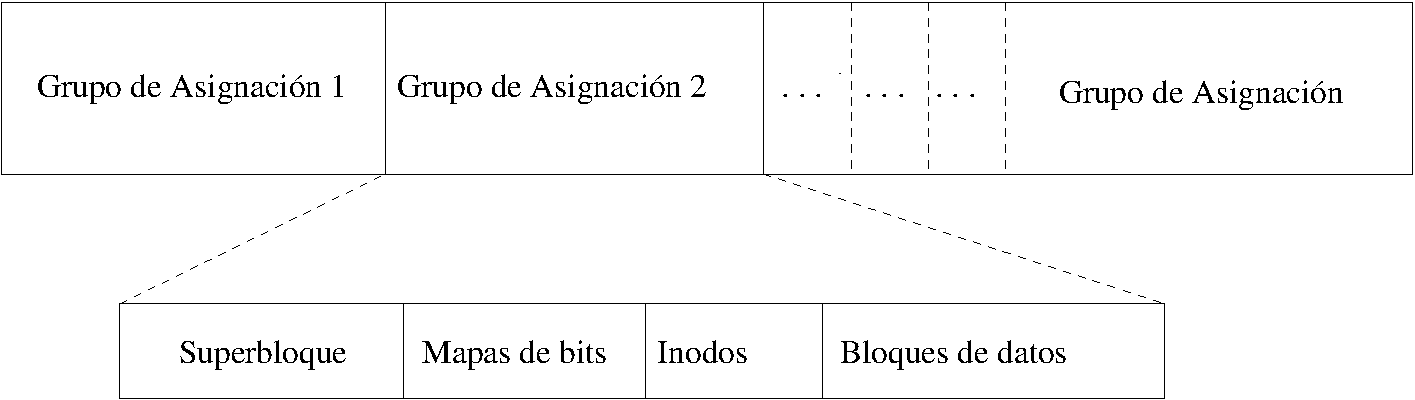
\includegraphics[width=1\linewidth]{figures/xfs.pdf}
    \caption{Organización lógica de XFS}
    \label{fig:organización lógica XFS}
\end{figure}

\begin{itemize}
    \item \textbf{Mapas de bits:} XFS utiliza mapas de bits para gestionar el estado de cada bloque en el grupo de asignación, lo que permite una gestión precisa y eficaz del espacio de almacenamiento.

    \item \textbf{Inodos:} En XFS, al igual que en los demás sistemas de ficheros analizados, los inodos representan archivos, directorios y pipes, almacenando información vital como permisos, propietarios, tamaño y ubicación de los datos del archivo. Sin embargo, los inodos en XFS tienen características especiales que los distinguen. En particular, XFS utiliza inodos extendidos, los cuales pueden almacenar atributos adicionales y extensiones de metadatos. Además, XFS implementa un esquema avanzado de asignación dinámica de inodos, contribuyendo a un rendimiento superior en operaciones de E/S y una mayor escalabilidad del sistema de ficheros.

    \item \textbf{Bloques de datos:} Los bloques de datos en XFS contienen los datos reales de los archivos y directorios, y pueden organizarse de diversas formas según las necesidades del sistema de ficheros. Esta flexibilidad en la organización de bloques de datos permite una adaptación óptima a diferentes cargas de trabajo y requisitos de almacenamiento.
\end{itemize}

\subsection{Características de XFS}

En cuanto a las características mencionadas anteriormente en la sección \ref{sec:caracteristicas_principales_sistemas_ficheros}, el sistema de ficheros XFS, al igual que EXT4 y BTRFS, ofrece una amplia gama de capacidades avanzadas. Entre estas características se incluyen el journaling para garantizar la integridad de los datos en caso de fallos del sistema. Sin embargo, no ofrece soporte nativo para snapshots, \textit{copy on write}, compresión o deduplicación. En cambio, ofrece las siguientes características:

\textbf{Administrador de Volúmenes XLV (Volume Manager XLV):} En el sistema de ficheros XFS, el administrador de volúmenes XLV proporciona una capa de abstracción adicional entre el sistema de ficheros y los dispositivos de almacenamiento físico. Pudiendo implementar configuraciones como \textit{striping}, \textit{mirroring} y \textit{concatenación} \cite{soltis2007xfs}.

El \textit{striping} distribuye equitativamente los datos entre varios discos, mejorando el rendimiento al permitir la lectura y escritura simultánea en múltiples dispositivos, especialmente en entornos de alta demanda. El \textit{mirroring} duplica la información en múltiples discos para aumentar la tolerancia a fallos y garantizar la integridad de los datos en XFS. Por otro lado, la \textit{concatenación} combina varios discos en un solo volumen lógico, facilitando la gestión eficiente de grandes cantidades de datos.

\textbf{Soporte para ACL y atributos extendidos:} XFS admite listas de control de acceso (ACL) y atributos extendidos, proporcionando una mayor funcionalidad en comparación con los permisos básicos de la máscara UGO. Estas características permiten una gestión más detallada de los permisos de acceso, así como el almacenamiento de información adicional asociada con los archivos y directorios, ofreciendo un control más preciso y enriquecido sobre la seguridad y los metadatos.

\textbf{Optimización para acceso paralelo:} Una de las características distintivas de XFS es su habilidad para dividir el espacio de almacenamiento en grupos de asignación independientes. Esta funcionalidad crea un entorno propicio para realizar operaciones de entrada/salida (E/S) de manera simultánea y eficiente. No solo acelera de manera significativa el rendimiento del sistema de ficheros, sino que también permite la ejecución paralela de múltiples operaciones de lectura y escritura, mejorando así la eficacia y capacidad de respuesta del sistema.

\section{ZFS (Zettabyte File System)}

ZFS es un sistema de ficheros transaccional diseñado para garantizar la integridad de los datos en todo momento. A diferencia de los sistemas de ficheros tradicionales que sobrescriben datos in situ y pueden dejar el sistema en un estado incoherente en caso de fallos, ZFS utiliza un enfoque transaccional completo. Lo que asegura que el estado del sistema de ficheros siempre sea coherente en disco.

\subsection{Estructura interna de ZFS}

La funcionalidad y organización del sistema de ficheros ZFS se presentan detalladamente en la figura \ref{fig:estructura ZFS}. Este diagrama proporciona una visión completa de cómo se relacionan los discos con los distintos elementos de abstracción específicos de ZFS. 

\begin{figure}[h!]
    \centering
    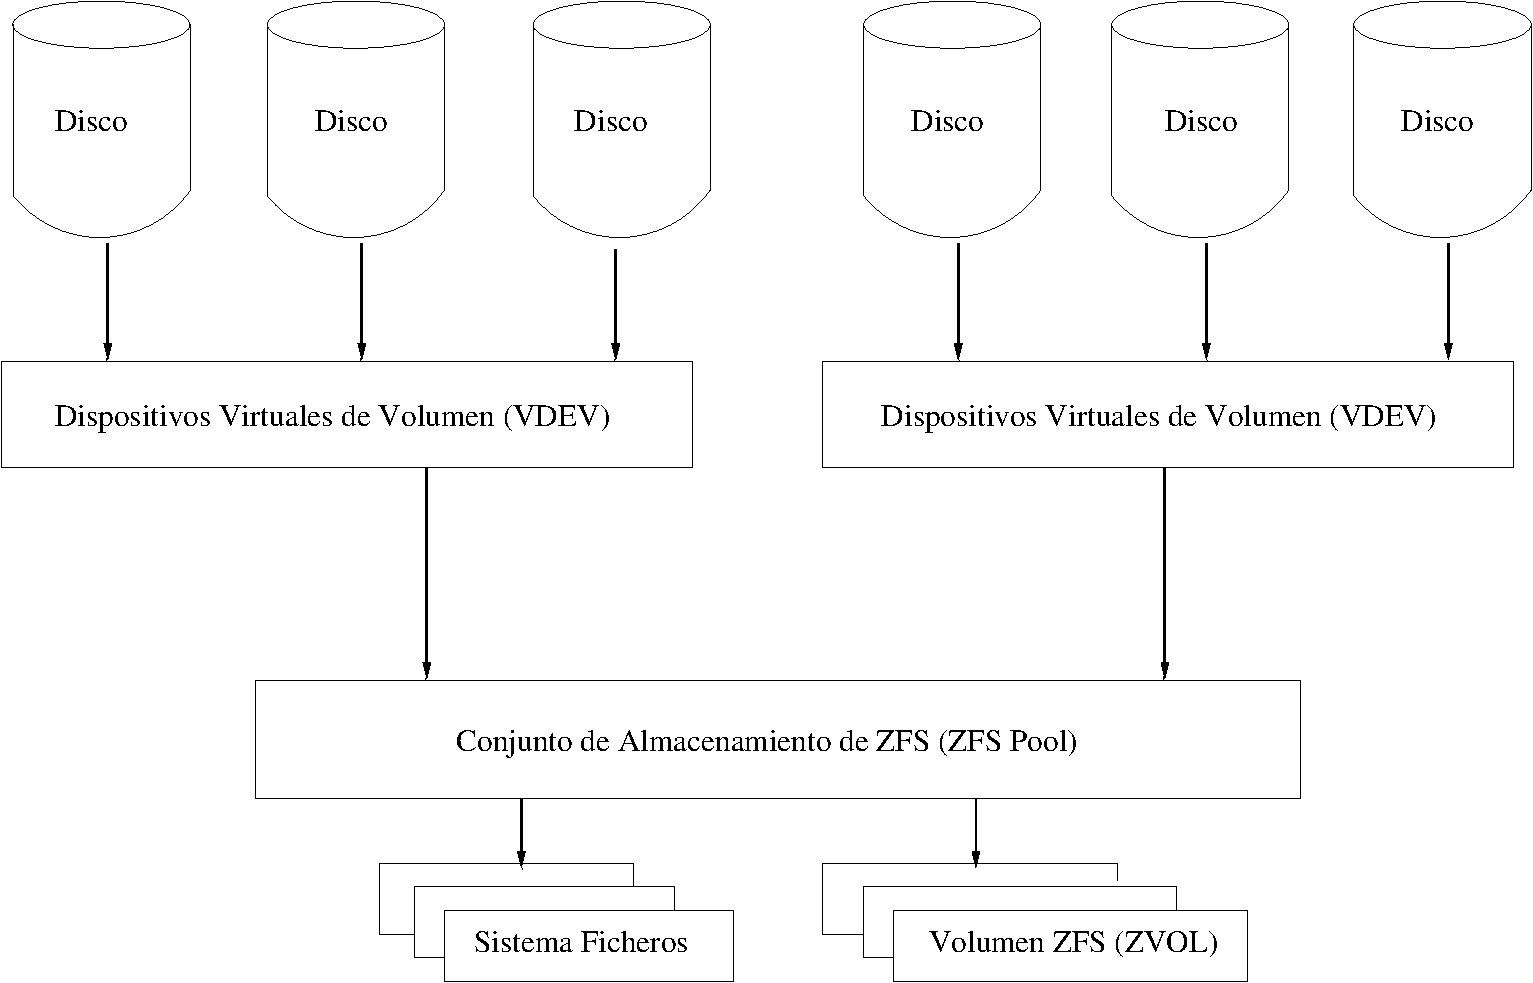
\includegraphics[width=1\linewidth]{figures/zfs.pdf}
    \caption{Organización del sistema de ficheros ZFS}
    \label{fig:estructura ZFS}
\end{figure}

\begin{itemize}
    \item \textbf{Zpool:} La unidad de almacenamiento de más alto nivel en ZFS. Un zpool puede consistir en uno o varios dispositivos de almacenamiento físicos como discos duros o SSDs, incluyendo configuraciones sobre dispositivos de almacenamiento en red.
    \item \textbf{Vdevs (Virtual Devices):} Los Vdevs son los bloques constructivos de un zpool, proporcionando la capacidad de agrupar dispositivos físicos para mejorar la redundancia y el rendimiento.
    \item \textbf{Datasets:} Conjuntos de datos que contienen información y metadatos, que pueden ser sistemas de archivos, volúmenes o instantáneas. Los datasets heredan propiedades del zpool pero también pueden tener configuraciones específicas como límites de espacio, compresión y deduplicación.
    \item \textbf{Zvols (ZFS Volumes):} Volumen de almacenamiento que simula un dispositivo de bloque, permitiendo el uso de aplicaciones que necesitan un sistema de ficheros convencional.
\end{itemize}

\subsection{Características de ZFS}

\textbf{Gestión de volúmenes integrada:} ZFS simplifica la gestión de volúmenes al combinar funciones de sistema de ficheros y administración de volúmenes en un único conjunto de herramientas. Soporta configuraciones RAID-Z, que ofrecen redundancia y tolerancia a fallos similar a RAID, pero con características avanzadas.\newline
    
\textbf{Integridad de datos con checksums:} ZFS garantiza la integridad de los datos mediante el uso de checksums. Cada bloque de datos contiene un checksum que se verifica durante las operaciones de lectura, facilitando la detección y corrección de errores silenciosos en los datos almacenados.\newline
    
\textbf{Conciencia de SSD/NVMe:} ZFS es consciente de las características de las tecnologías SSD/NVMe, aprovechando el soporte de TRIM/Discard, detalladas en la sección \ref{sec:caracteristicas_principales_sistemas_ficheros}. Esto optimiza las operaciones de almacenamiento, mejora el rendimiento general y contribuye a prolongar la vida útil de los dispositivos de almacenamiento flash.\newline
    
\textbf{Algoritmos de reparación automática:} En configuraciones RAID-Z, ZFS utiliza información de paridad para realizar reparaciones automáticas de datos corruptos, mejorando la fiabilidad del sistema de ficheros y protegiendo contra pérdidas de datos.\newline

\textbf{Soporte para modo zonificado:} ZFS es compatible con el modo zonificado, al igual que con BTRFS, se trata de una técnica de asignación de bloques adaptada a dispositivos de almacenamiento SMR/ZBC/ZNS. Esto mejora la eficiencia en la gestión de datos en entornos de almacenamiento zonificado.





